\documentclass{article}
\usepackage[utf8]{inputenc}
\usepackage{graphicx}

\usepackage{newpxtext,newpxmath}
\usepackage[
backend=biber,
style=alphabetic,
citestyle=alphabetic,
]{biblatex}
\addbibresource{bib.bib}

\usepackage{hyperref}
\hypersetup{
    colorlinks=true,
    linkcolor=blue,
    filecolor=magenta,      
    urlcolor=cyan,
    citecolor=blue,
    pdftitle={Multi-Splay Trees and Tango Trees},
    pdfpagemode=FullScreen,
}

\title{Multi-Splay Trees and Tango Trees}
\author{Christian Altamirano and Parker Rule}
\date{May 18, 2021}

\newcommand{\OPT}{\text{OPT}}

\begin{document}

\maketitle

\section{Introduction and literature review}
This project is an exploration of two data structures developed in the study of \emph{dynamic optimality}. Recall that a binary search tree is \emph{dynamically optimal} if, for every access sequence $X$, the tree executes the sequence in $O(\OPT(X))$ operations, where $\OPT(X)$ is the minimum number of unit-cost operations required to access $X$ in \emph{any} binary search tree \cite{demaine2007dynamic}. Splay trees \cite{sleator1985self} are conjectured to be dynamically optimal, but this conjecture is still unresolved after nearly four decades. However, several binary search trees have been shown to achieve $O(\log \log n \cdot OPT(X))$ performance---that is, they are $O(\log \log n)$-competitive. (Every balanced binary search tree is trivially $O(\log n)$-competitive.) Tango trees \cite{demaine2007dynamic} and multi-splay trees \cite{sleator2004dynamic, daniel2006log, derryberry2009properties} both achieve $O(\log \log n)$-competitiveness by encoding \emph{preferred paths} as trees of size $O(\log n)$ within a tree-of-trees representation. We have implemented multi-splay trees and made significant progress in the implementation of tango trees.

\section{Multi-splay implementation}
At a high level, a multi-splay tree is a tree made of splay trees where nodes have several augmentations. Each node has a \textit{marked} bit that tells whether or not this node is a root of its own splay tree. Splaying is done at the splay subtree level by rotating up until reaching a marked node.

Our implementation follows the C++ starter code shown in the appendix in \cite{sleator2004dynamic}, with a few modifications. First, in our implementation we don't include a few of the augmentations and instead compute some properties on the fly. This extra computation seems to cause at most a constant overhead for the runtime, and our experiments show that the runtime matches the asymptotic bounds for $n \leq 2^{20}$. We also make a subtle modification the \texttt{Query} recursive function to deal with nodes with infinite keys. Finally, we splay the nodes top-down rather than bottom-up---splaying nodes bottom-up as originally described in \cite{sleator2004dynamic} appears to be incorrect, as top nodes would have their pointers modified improperly.

%All the cases where we needed to recompute these augmentations were whenever a node would rotate up or when a node's preferred child changes from left to right or viceversa. This turned out to make this implementation somewhat simple.

All trees implemented for this project use a common base implementation of \texttt{BST} and \texttt{BSTNode} \href{https://github.com/6851-2021/tango-trees/blob/master/src/bst.hpp}{(code)}. These classes provide a common interface for inserts, deletes, and queries and are generic over key, value, and metadata types.



\subsection{Benchmarks: splay trees vs. multi-splay trees} \label{section:benchmarks}
For testing, we use the universe made of keys in $[0, 2^{20} - 2]$ and sample random trees containing all of these keys. (We insert elements in random order to avoid starting with a pathological splay tree.)  For splay trees \href{https://github.com/6851-2021/tango-trees/blob/master/src/splay.hpp}{(code)}, we simply insert all the possible keys to an empty tree and then perform random queries. For multi-splay trees \href{https://github.com/6851-2021/tango-trees/blob/master/src/multisplay.hpp}{(code)}, we make a perfect binary search tree and perform random queries to modify all the preferred children. After this initialization, we test how multi-splay trees perform compared to splay trees using several query sequences \href{https://github.com/6851-2021/tango-trees/blob/master/main.cc}{(code)}. 

For our benchmarks, we used the sequence of all keys in increasing order, a sequence of random keys, and a sequence of all keys in bit reversal order. It is known that for a bit reversal sequence $X$ of length $n$, $\OPT(X) = \Theta(n \log n)$ \cite{wilber1989lower}.

Our results show that multi-splay tree queries seem to take $O(\log n)$ amortized time per query, which matches the asymptotic bounds in \cite{sleator2004dynamic}. Querying the increasing sequence is much faster than a random sequence. Asymptotically, sequential accesses in splay trees run in linear time \cite{tarjan1985sequential}. Our experiments also show that for the increasing sequence query, the number of rotations needed is linear, always less than $3.8N$ for $N = 2^{20}-1$. This matches the results in \cite{sleator2004dynamic}.

\begin{figure}[h!]
    \centering
    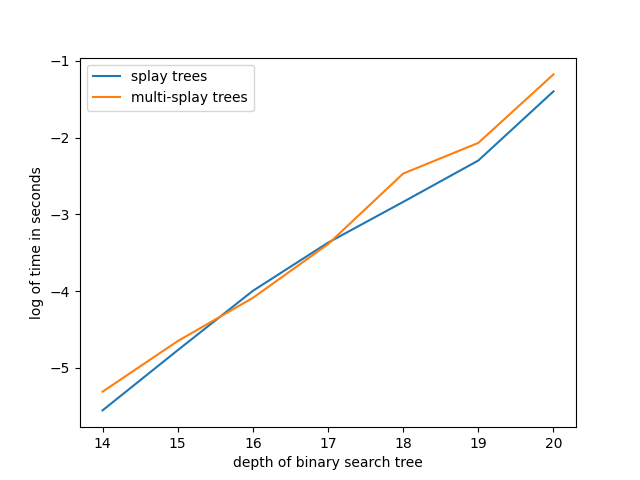
\includegraphics[width = 10cm]{increasing}
    \caption{Increasing sequence query.}
    \label{fig:my_label}
\end{figure}

\begin{figure}[h!]
    \centering
    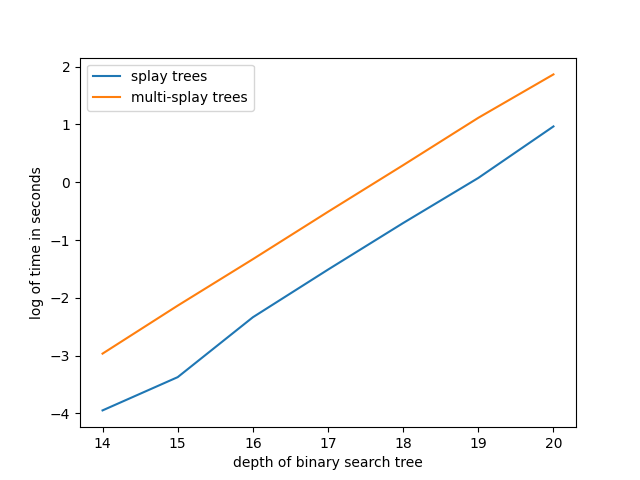
\includegraphics[width = 10cm]{random}
    \caption{Random sequence query.}
    \label{fig:my_label}
\end{figure}

\begin{figure}[h!]
    \centering
    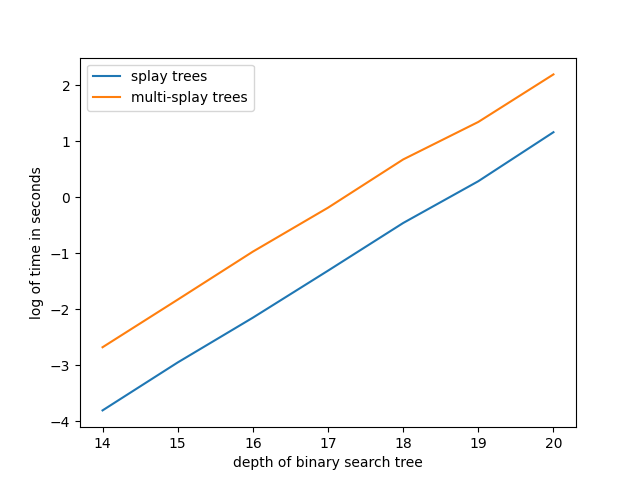
\includegraphics[width = 10cm]{reversal}
    \caption{Bit reversal sequence query.}
    \label{fig:my_label}
\end{figure}


% \begin{center}
% \begin{tabular}{|c|c|c|c|c|}
% \hline
% & sequential & Random & Decreasing \\
% \hline
% Splay trees &0.066064 & 1.04084& 0.068608 \\
% \hline
% Multi-splay trees & 0.27566& 7.56731 & 0.281041 \\
% \hline
% \end{tabular}
% \end{center}

% The following table shows the how many rotations were performed for each query sequence for each type of tree 

% \begin{center}
% \begin{tabular}{|c|c|c|c|c|}
% \hline
% & sequential & Random & Decreasing \\
% \hline
% Splay trees & 1337436&13681726 & 1336175 \\
% \hline
% Multi-splay trees &3709955 & 63218515& 3768030 \\
% \hline
% \end{tabular}
% \end{center}

\section{Partial tango implementation and future work}
The implementation details of tango trees are significantly more subtle than those of multi-splay trees, even though the data structures are conceptually similar. In \cite{demaine2007dynamic}, an augmented red-black tree is used as the basis of the tree-of-trees representation. For standard red-black tree implementation details, including split and concatenate operations, we follow \cite{tarjan1983data, sedgewick1990algorithms, cormen2009introduction, wein2005efficient, wiki:rb}. \emph{Marked nodes} represent the roots of individual trees, and the red-black invariants are maintained separately within each of these trees, and all of the standard tree operations---such as rotations and height queries---must be updated to respect marking. In most cases, marked nodes should be treated as null pointers (though preserved in rotations), but this rule can be problematic when the main root is marked. Additionally, \cite{demaine2007dynamic} requires nodes to be augmented with the minimum and maximum perfect depths within their subtrees, and these augmentations must be updated at each tree operation while respecting marked nodes. (Nodes also store their fixed depths in the perfect tree.) In our implementation, we reuse the base \texttt{BST} and \texttt{BSTNode} classes \href{https://github.com/6851-2021/tango-trees/blob/master/src/bst.hpp}{(code)} used in the multi-splay tree implementation.

As \cite{demaine2007dynamic} describes tango trees for a static universe of keys, we add root-level \texttt{lock()} and \texttt{unlock()} operations. In the unlocked phase, the tree supports inserts and deletes (handled lazily), but not queries; in the locked phase, the tree is converted to a tango tree and allows only queries. The tree is rebuilt into a perfect tree at each lock and unlock operation.

Unfortunately, our implementation \href{https://github.com/6851-2021/tango-trees/blob/master/src/rb.hpp}{(code)} is incomplete; implementing tree operations that respect the nuances of marked nodes proved more difficult than anticipated under our time constraints. However, we believe that our work may be a useful starting point for future 6.851-ers. To this end, we list the next steps necessary to complete the implementation below.

\subsection{Completed tasks}
\begin{itemize}
    \item \textbf{Base red-black tree implementation}, as described in \cite{cormen2009introduction}.
    \item \textbf{Perfect tree rebuilding.} After an initial series of inserts and deletes, we lock the tree and rebuild into a perfect tree in the obvious recursive way. We update each node's metadata and record perfect depths.
    \item \textbf{Split and concatenate operations.} These operations are distinct from the standard split and join operations used to implement set operations in C++ in two ways: both operations must respect marked nodes, and the \texttt{concatenate()} operation is a special case of the general join operation where the trees to be joined share a root in the tree of trees.
    \item \textbf{Tree augmentation.} We recompute minimum and maximum depths in each subtree as necessary (this entails following parent pointers up to marked nodes). 
\end{itemize}

\subsection{Future work}
\begin{itemize}
    \item \textbf{$P_i \to T_i$ conversion.} One major advantage of multi-splay trees is that (up to marking) a splay tree is also a valid multi-splay tree. However, this is not the case for nontrivial tango trees---after rebuilding an arbitrary red-black tree to form a perfects tree, we must additionally ``tangoize'' by converting the perfect tree representation $P_i$ to a tree-of-trees representation $T_i$. Of course, $T_i$ is determined by both the elements in $P_i$ and a preferred path through $P_i$. It would suffice to hardcode an initial element to access (say, the leftmost element) as the last step in \texttt{lock()}.
    \item \textbf{Full cut and join operations.} We have implemented a basic version of the \texttt{cut()} operation but have not thoroughly tested it due to the lack of $P_i \to T_i$ conversion. (The \texttt{join()} operation is largely symmetric.)
    \item \textbf{Tango algorithm.} This is simply the application of \texttt{cut()} and \texttt{join()} operations to reflect preferred path changes.
    \item \textbf{Thorough tests and invariant checks.} The implicit tree-of-tree representation has a number of complicated tree invariants (it typically contains many red-black trees of differing height); globally, it must correspond to a valid preferred path and be a valid binary search tree.
\end{itemize}

Beyond these implementation steps, there are a number of interesting possible extensions.\footnote{Inspired by \cite{okasaki1999purely}, we briefly considered using a purely functional language such as Haskell, which would likely yield a more compact representation of the tree operations. However, it is not clear that the trees' asymptotic performance guarantees would remain the same in an immutable setting.} It would be informative to extend the benchmarks in section \ref{section:benchmarks} to directly compare multi-splay trees and tango trees. It is known that the tango algorithm runs in $\Theta(\log n \log \log n)$ time per query for random access sequences \cite{daniel2006log}, but perhaps there are sequences (such as sequential or near-sequential access) for which they perform similarly in practice. 


\section*{Acknowledgements}
We thank George Tang and Sebastian Mendez for contributing some early scaffolding code to this project.


%\subsection{Future work}

\newpage
\printbibliography


% TODO: references

\end{document}
